
\newpage
{\bfseries МРНТИ 20.23.17}; 20.53.21


\sectionwithauthors{А.С. Сейтенов, Т.К. Жукабаева, S. Al-Majeed, C. Wolff}{РАЗРАБОТКА МИС СИСТЕМЫ ТЕЛЕМЕДИЦИНЫ ДЛЯ ЗАПИСИ К МЕДИЦИНСКИМ
СПЕЦИАЛИСТАМ}
\begin{center}

{\bfseries \textsuperscript{1, 2,4}А.С. Сейтенов\textsuperscript{🖂},
\textsuperscript{1}Т.К. Жукабаева, \textsuperscript{3}S. Al-Majeed,
\textsuperscript{4}C. Wolff}

\textsuperscript{1} Евразийский национальный университет имени Л.Н.
Гумилева, Астана, Казахстан,

\textsuperscript{2}Astana IT University, Астана, Казахстан,

\textsuperscript{3}Al Akhawayn University, Ифран, Марокко,

\textsuperscript{4}Fachhochschule Dortmund, Дортмунд, Германия

Корреспондент-автор: \emph{altynbekss@gmail.com}
\end{center}

Технологии телемедицины стремительно развиваются, предоставляя новые
возможности удаленного медицинского обслуживания, особенно в условиях
ограниченного доступа к медицинским учреждениям. Разработка Медицинской
Информационной Системы (МИС) для телемедицины становится важной задачей,
направленной на улучшение качества медицинских услуг, оптимизацию
административных процессов и повышение доступности квалифицированной
медицинской помощи для широкого круга пациентов, включая тех, кто
проживает в отдаленных районах. В данной научной работе проведен
детальный анализ для подбора среди существующих методов и технологий в
этой области, а также предложены новые, инновационные подходы к решению
актуальных проблем, связанных с внедрением МИС в практику. Результаты
исследования могут быть полезны для разработчиков и внедренцев МИС,
руководителей учреждений здравоохранения, а также для исследователей,
занимающихся вопросами телемедицины и информационных технологий в
здравоохранении. Предложенные подходы и рекомендации способствуют
улучшению процессов предоставления медицинских услуг, повышению
эффективности телемедицины в целом и улучшению взаимодействия между
врачами и пациентами на всех уровнях медицинского обслуживания.

{\bfseries Ключевые слова}: телемедицина, система телемедицины; удаленное
медицинское обслуживание; медицинская информационная система; удаленная
запись; электронный прием пациента; приложение.
\begin{center}

{\bfseries ТЕЛЕМЕДИЦИНАЛЫҚ МАМАНДАРҒА ТІРКЕЛУ ҮШІН МАЖ ЖҮЙЕСІН ДАМЫТУ}

{\bfseries \textsuperscript{1, 2,4}А.С. Сейтенов\textsuperscript{🖂},
\textsuperscript{1}Т.К. Жукабаева, \textsuperscript{3}S. Al-Majeed,
\textsuperscript{4}C. Wolff}

\textsuperscript{1}Л.Н. Гумилев атындағы Еуразия ұлттық университеті,
Астана, Қазақстан,

\textsuperscript{2} Astana IT University, Астана, Қазақстан,

\textsuperscript{3}Al Akhawayn University, Ифран, Марокко,

\textsuperscript{4}Fachhochschule Dortmund, Дортмунд, Германия

e-mail: altynbekss@gmail.com
\end{center}

Телемедицина технологиялары тез дамып келеді, медициналық қызметтерге
қашықтықтан қол жеткізудің жаңа мүмкіндіктерін ұсынады, әсіресе
медициналық мекемелерге кіру шектеулі болған жағдайда. Телемедицина үшін
Медициналық Ақпараттық Жүйенің (МАЖ) әзірлемесі медициналық қызметтердің
сапасын жақсартуға, әкімшілік процестерді оңтайландыруға және жоғары
білікті медициналық көмекті кең ауқымды пациенттерге, соның ішінде
шалғай аудандарда тұратындарға қолжетімділікті арттыруға бағытталған
маңызды міндет болып табылады. Осы ғылыми жұмыста қазіргі уақытта
қолданылып жүрген әдістер мен технологияларды талдау жүргізілді,
сондай-ақ МАЖ-ді практикаға енгізу мәселелерін шешуге арналған жаңа,
инновациялық тәсілдер ұсынылды. Зерттеу нәтижелері МАЖ әзірлеушілері мен
енгізушілеріне, денсаулық сақтау мекемелерінің басшыларына, сондай-ақ
телемедицина мен денсаулық сақтау ақпараттық технологиялары
мәселелерімен айналысатын зерттеушілерге пайдалы болуы мүмкін. Ұсынылған
тәсілдер мен ұсыныстар медициналық қызмет көрсету процестерін
жақсартуға, телемедицина тиімділігін арттыруға және дәрігерлер мен
пациенттер арасындағы өзара әрекеттесуді барлық медициналық қызмет
көрсету деңгейлерінде жақсартуға ықпал етеді.

{\bfseries Түйін сөздер}: телемедицина, телемедицина жүйесі, қашықтықтан
медициналық қызмет көрсету, медициналық ақпараттық жүйе, қашықтықтан
тіркеу, электронды пациент қабылдау, қосымша.
\begin{center}

{\bfseries DEVELOPMENT OF MIS TELEMEDICINE SYSTEM FOR APPOINTMENT WITH
MEDICAL SPECIALISTS}

{\bfseries \textsuperscript{1,2,4}A.S. Seitenov\textsuperscript{🖂},
\textsuperscript{1}T.K. Zhukabayeva, \textsuperscript{3}S. Al-Majeed,
\textsuperscript{4}C. Wolff}

\textsuperscript{1} L.N. Gumilyov Eurasian National University, Astana,
Kazakhstan,

\textsuperscript{2} Astana IT University, Astana, Kazakhstan,

\textsuperscript{3} Al Akhawayn University, Ifrane, Morocco,

\textsuperscript{4} Fachhochschule Dortmund, Dortmund, Germany,

e-mail: altynbekss@gmail.com
\end{center}

Telemedicine technologies are rapidly evolving, providing new
opportunities for remote medical care, especially in areas with limited
access to medical facilities. Developing a Medical Information System
(MIS) for telemedicine is becoming a crucial task aimed at improving the
quality of medical services, optimizing administrative processes, and
enhancing the availability of qualified medical care for a broad range
of patients, including those living in remote areas. This research paper
provides a detailed analysis of existing methods and technologies in
this field and proposes new, innovative approaches to addressing the
current challenges associated with implementing MIS in practice. The
findings may be useful for MIS developers and implementers, healthcare
facility managers, and researchers involved in telemedicine and
healthcare information technology. The proposed approaches and
recommendations contribute to improving medical service delivery
processes, increasing the overall effectiveness of telemedicine, and
enhancing interactions between doctors and patients at all levels of
medical care.

{\bfseries Keywords}: telemedicine, telemedicine system, remote medical
service, medical information system, remote registration, electronic
patient reception, application.

{\bfseries Введение.} В последние годы телемедицина стала одним из наиболее
быстро развивающихся направлений в области здравоохранения, предоставляя
возможности удаленного медицинского обслуживания и консультаций.
Разработка МИС (Медицинская информационная система) для телемедицины
представляет собой важную задачу, поскольку такие системы обеспечивают
управление медицинскими данными, улучшение качества обслуживания
пациентов и оптимизацию административных процессов. Обоснование выбора
данной темы основывается на опыте предшественников, которые подчеркивают
необходимость интеграции информационных технологий в медицину для
повышения эффективности и доступности медицинских услуг {[}1, 2{]}.

Актуальность разработки МИС для телемедицины определяется высоким
интересом к инновационным методам предоставления медицинской помощи и
глобальными тенденциями цифровизации здравоохранения. Пандемия COVID-19
значительно усилила потребность в удаленных медицинских услугах, что в
свою очередь требует эффективных информационных систем для обеспечения
качества и непрерывности медицинского обслуживания {[}2, 3{]}.
Значимость данной темы заключается в развитии научного понимания
принципов построения и функционирования МИС для телемедицины, а так же в
непосредственном улучшении качества медицинских услуг и управлении
ресурсами здравоохранения {[}3, 4{]}.

Многие зарубежные исследования показывают, что эффективные системы
регистрации пациентов и управления данными в телемедицине играют
ключевую роль в обеспечении доступности и качества медицинских услуг.
Например, исследования показывают, что использование телемедицины для
управления хроническими заболеваниями, такими как диабет и гипертония,
значительно улучшает показатели здоровья пациентов и снижает нагрузку на
медицинские учреждения. Кроме того, современные цифровые системы, такие
как электронные медицинские записи и телемедицинские консультации,
способствуют более эффективному взаимодействию между пациентами и
медицинскими специалистами, улучшая качество обслуживания и
удовлетворенность пациентов {[}5, 6{]}.

Цель данной научной работы состоит в разработке и представлении
архитектуры и модели МИС системы для записи к специалистам, а также в
анализе существующих технологий в этой области. Для достижения этой цели
необходимо решить следующие задачи: провести анализ произведенных
исследований, определить сильные стороны существующих решений, а также
предложить новые подходы к решению проблем.

Значение данной научной работы заключается в том, что ее результаты
могут быть полезны для разработчиков и внедренцев МИС, руководителей
здравоохранения, а также для исследователей, занимающихся проблемами
телемедицины и информационных технологий в здравоохранении. Предложенные
подходы и рекомендации могут способствовать улучшению процессов
предоставления медицинских услуг и повышению эффективности телемедицины
в целом.

{\bfseries Материалы и методы.} Разработка и внедрение медицинских
информационных систем (МИС) в сфере телемедицины активно изучается в
последние годы. Эти системы предназначены для улучшения результатов
лечения пациентов, оптимизации процессов здравоохранения и более
эффективного распределения ресурсов. В данном разделе рассмотрены
основные направления и результаты исследований в этой области {[}5,
6{]}.

Экосистема телемедицины подразумевает вовлечение использования
информационных и коммуникационных технологий для упрощения
предоставления медицинских услуг на расстоянии. Платформа данной
технологий может состоять из следующих сервисов: дистанционная
консультация, мониторинг состояния здоровья пациента, обмен медицинской
информацией между специалистом и пациентом, а также между специалистами.
Развитие телемедицины связано с необходимостью преодоления
географических, социальных и экономических барьеров, что особенно
актуально для удаленных и малонаселенных регионов {[}7, 8{]}.

Исследования показывают, что МИС могут значительно улучшить координацию
ухода и ускорить процессы принятия решений в здравоохранении. Системы,
основанные на таких технологиях, как интернет вещей (IoT), искусственный
интеллект (AI) и большие данные (Big Data), предлагают новые возможности
для телемедицины, включая удаленный мониторинг пациентов,
прогнозирование эпидемий и поддержку врачебных решений {[}8-10{]}.

Внедрение телемедицины и МИС активно продвигалось в условиях пандемии
COVID-19, что продемонстрировало их потенциал в условиях кризиса.
Современные технологии, такие как облачные серверы, позволяют передавать
большие объемы данных с минимальной задержкой, что является критически
важным для развития телемедицины {[}8,9{]}.

Кроме того, исследования показывают, что несмотря на значительные
преимущества, внедрение телемедицины сталкивается с рядом проблем,
включая необходимость значительных инвестиций в инфраструктуру и
обучение персонала, а также вопросы безопасности данных {[}10{]}.
Однако, в долгосрочной перспективе, успешная интеграция МИС и
телемедицины может привести к значительным улучшениям в доступности и
качестве медицинской помощи, особенно в отдаленных регионах {[}7-9{]}.

Помимо вышеуказанного замечания для разработки системы для телемедицины
необходимо учитывать этические аспекты реализации. Такие как обеспечение
конфиденциальности и передачи информации о пациенте, требуют тщательного
рассмотрения при разработке и внедрении телемедицинских систем {[}10,
11{]}.

Несмотря на эти проблемы, телемедицина имеет значительный потенциал для
улучшения качества медицинской помощи. Одним из ключевых преимуществ
является возможность предоставления специализированных медицинских услуг
в отдаленные и сельские районы, где доступ к квалифицированным
медицинским кадрам ограничен {[}8,12{]}. Исследования показывают, что
телемедицинские консультации могут быть столь же эффективны, как и
традиционные очные визиты, в диагностике и лечении ряда заболеваний
{[}13{]}. Более того, телемедицина может способствовать снижению затрат
на медицинское обслуживание, уменьшая необходимость транспортировки
пациентов и сокращая время ожидания для получения медицинской помощи
{[}14{]}.

В дополнении, реализация и запуск медицинской информационной системой
для телемедицины позволяет улучшить координацию ухода за пациентами,
облегчая обмен медицинской информацией между различными учреждениями и
специалистами. Это особенно важно для пациентов с хроническими
заболеваниями, требующими постоянного мониторинга и координации
различных видов лечения {[}15{]}. Кроме того, использование телемедицины
в сочетании с МИС может улучшить сбор и анализ медицинских данных, что
способствует проведению более точных и обоснованных клинических
исследований {[}16{]}.

В рамках данного исследования в статье представлена архитектура и модель
медицинской информационной системы для телемедицины, включающую функцию
электронной записи к специалистам. Исследовательская работа учитывает
анализ, произведенный в работах {[}7{]}. Анализ рассматривал
существующую платформу и бизнес-процессы, зарегистрированных в перечне
МИС Министерства здравоохранения Республики Казахстан, позволит
определить сильные и слабые стороны текущих решений.

Основная задача разработки модели МИС --- создание интуитивно понятный и
удобный инструмент для оптимизации взаимодействия врачей и пациентов. На
первом этапе необходимо оптимизировать процессы обмена информацией, что
включает разработку удобных интерфейсов. Важно подобрать подходящие
технологии и решения для обеспечения легкости и эффективности
коммуникации между пользователями системы. К тому же исследованы подходы
для упрощения записи на прием, включая создание системы
автоматизированного бронирования и управления расписанием врачей.
Изучены существующие методы и инструменты, а также оценена их
применимость в проекте {[}17{]}.

Для реализации МИС исследованы современные технологии и оборудование.
Изучены фреймворки, такие как Django, для обеспечения надежности
системы. Для разработки интерфейса оценены инструменты Angular, для
обеспечения интерактивности и удобства. Рассмотрены базы данных, включая
SQLite, с точки зрения производительности,

Интерфейс играет ключевую роль в веб-приложении, обеспечивая удобство
поиска врачей, записи на прием и проведения онлайн-консультаций в
реальном времени. Необходима интуитивно понятная и простая в
использовании интеграция, для чего Angular является оптимальным
решением.

\begin{figure}[H]
	\centering
	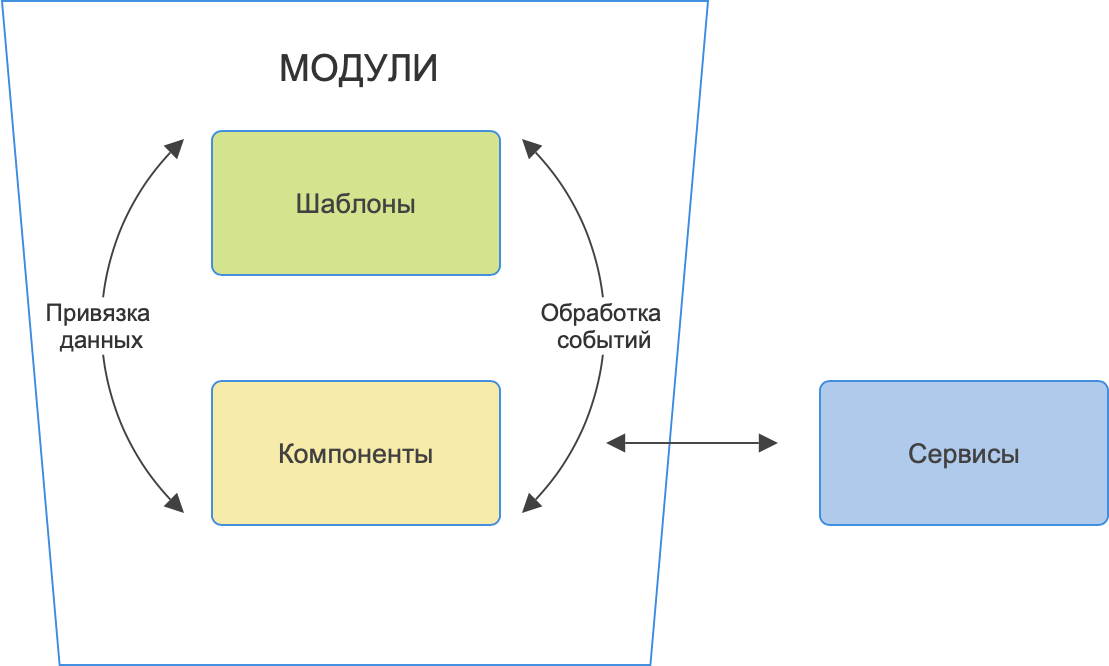
\includegraphics[width=0.8\textwidth]{assets/151}
	\caption*{}
\end{figure}

{\bfseries Рис. 1 - Архитектура Angular}

Архитектура в Angular на Рисунке 1 построена на компонентах, где каждый
компонент включает свою логику, данные и представление. Компоненты
(Component) представляют элементарные части приложения, включающие
HTML-шаблоны, CSS для стилей и TypeScript для логики, позволяя
управление каждой частью, делая их независимыми модулями для реализации
МИС системы. Сервисы (Services) выполняют задачи: получение данных о
пациенте, работа с учетными записями и управление встречами, позволяя
компонентам заниматься на представлении информации пользователя
{[}18{]}.

Модули (Modules) объединяют схожие компоненты и сервисы, предлагая
функции такие, как личная консультация между врачом и пациентом в
отдельный блок. Маршрутизация (Routing) позволяет перемещаться между
страницами приложения, такими как вход, регистрация, просмотр врачей и
запись на прием. Привязка данных (Data binding) и обработка событий
(event handling) автоматически обновляет интерфейс при изменении
состояния приложения. Обработка событий позволяет компонентам
реагировать на действия пациентам, такие как отправка формы заявки или
нажатие кнопки, обеспечивая оперативное взаимодействие {[}18{]}.

Выбранная методология соответствует целям проекта, поскольку направлена
на тщательное исследование, практическую разработку и эффективную
интеграцию функций. Сочетание обзоров литературы и выбранной методологии
обеспечило понимание потребностей пользователей и существующих решений.

{\bfseries Результаты и обсуждение.} Выбор остановился на SQLite для базы
данных из-за её легкости и интеграции с Django фреймворком. SQLite
предлагает простоту и удобство, позволяя сосредоточиться на разработке
без сложной настройки. В дальнейшем система может плавно перейти на
более масштабируемое решение, поддерживаемое Django, благодаря гибкости
SQLite {[}19{]}.

На рисунке 2 представлена схема базы данных (БД) МИС системы. База
данных содержит данные о врачах и пациентах, организуя информацию в
нескольких таблицах. База данных содержит на таблицы, разделенных на три
основные группы (Доктор, Пациент, Запись).

\begin{figure}[H]
	\centering
	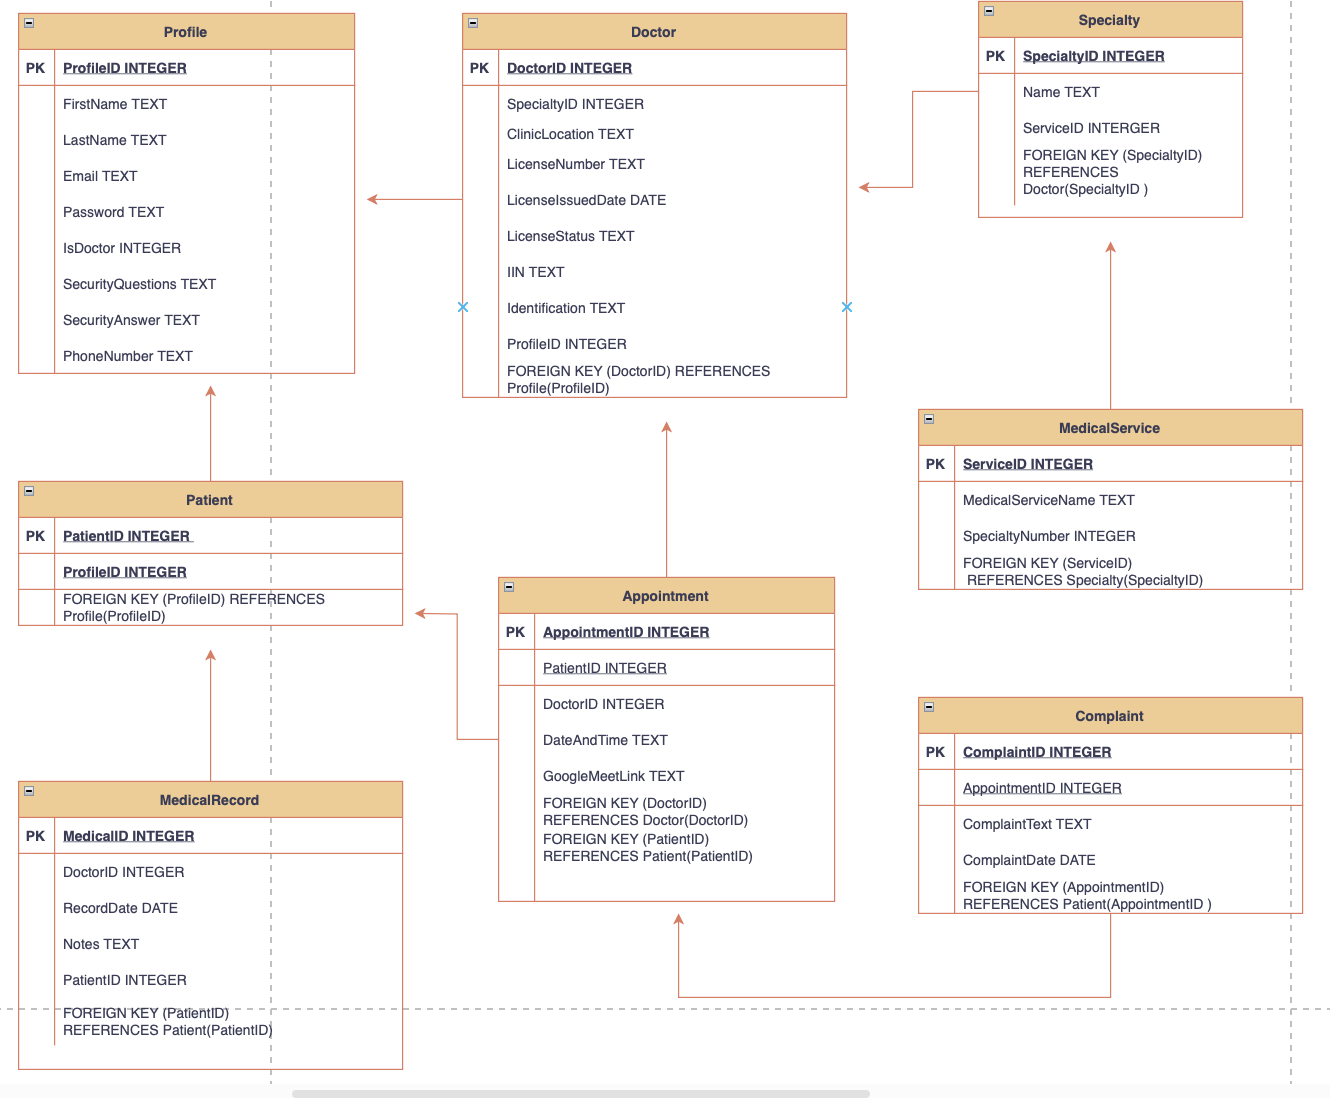
\includegraphics[width=0.9\textwidth]{assets/152}
	\caption*{\bfseries Рис. 2 -- ERD Диаграмма БД МИС системы}
\end{figure}


Профиль (Profile): Содержит основную информацию о пользователе, включая
имя, фамилию, адрес электронной почты, пароль, секретный вопрос и ответ
для верификации, а также индикатор статуса врача.

Доктор (Doctor): Предоставляет дополнительные данные, специфичными для
врачей, такими как специальность, расположение клиники, информация о
лицензии и статус проверки, если профиль является доктором.
Специальность (Specialty): Содержит информацию о врачебных
специальностях. Медицинские услуги (MedicalService) - тождествуется со
соответствующим лечебным специальностям.

Пациент: Расширяет таблицу "Профиль" для представления пациентов, если
запись о профиле является пациентом. Медицинская запись (MedicalRecord):
Сохраняет данные о пациентах.

Запись (Appointment): Управляет деталями встреч между врачами и
пациентами, включая дату, время и ссылку на онлайн-консультации. Жалоба
(Complaint): Обрабатывает жалобы пациентов предварительно до записи на
прием к врачу.

Рисунок 3 показывает структуру нашего бэкенда, организованного по
приложениям:

\begin{figure}[H]
	\centering
	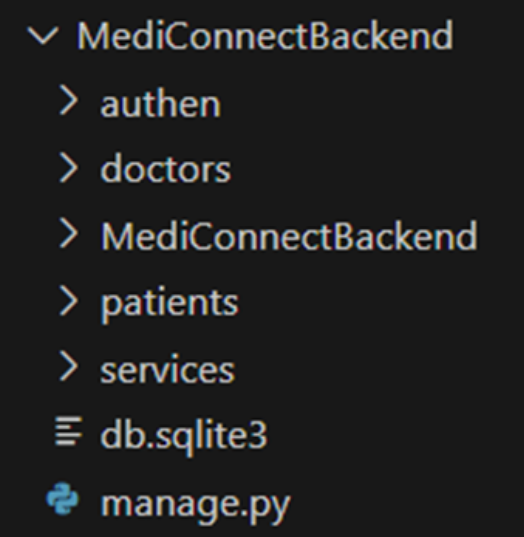
\includegraphics[width=0.3\textwidth]{assets/153}
	\caption*{\bfseries Рис. 3 - Структура бэкенда системы}
\end{figure}


Каждый модуль отвечает со следующие функции:

\begin{enumerate}
\def\labelenumi{\arabic{enumi}.}
\item
  Authen: Аутентификация и управление пользователями.
\item
  Врачи (doctors): Профили врачей, включая специальности и проверку
  лицензий.
\item
  Пациенты (patients): Профили пациентов и их взаимодействие с врачами.
\item
  Услуги (services):Управление медицинскими услугами и запись на прием.
\item
  MediConnectBackend: Основная программа с глобальными настройками и
  конфигурациями.
\end{enumerate}

В проекте запрос поступает к диспетчеру URL-адресов в `urls.py`, который
направляет его к соответствующему представлению в `views.py`.
Представление обрабатывает запрос, проверяет данные, вызывает
бизнес-логику и взаимодействует с моделями из `models.py`, управляющими
базой данных через Django. Для преобразования моделей в JSON и проверки
данных используются сериализаторы из `serializers.py`. После обработки
представление возвращает HTTP-ответ, будь то HTML-шаблон, JSON для API
или перенаправление, указанные на Рисунке 4.

\begin{figure}[H]
	\centering
	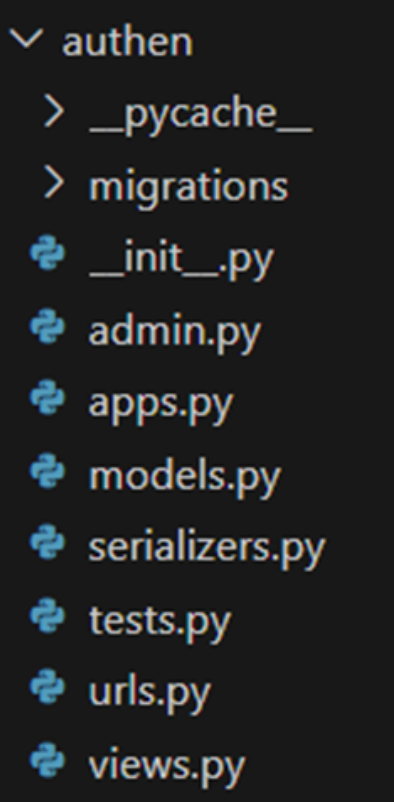
\includegraphics[width=0.2\textwidth]{assets/154}
	\caption*{\bfseries Рис. 4 - Структура программы}
\end{figure}


МИС система обеспечивает доступ к медицинским услугам, позволяя
пользователям искать и планировать встречи. Программа моделируют
специализации, медицинские услуги и посещения, где прием и медицинское
обслуживание соответствуют различным видам услуг. Функциональность,
связанная с доступом к услугам, созданием встреч и изменением данных о
бронировании, реализована в `view.py`.

Дизайн страницы входа позволяет существующим пользователям войти в
систему и обрабатывает данную функциональность, отображен на Рисунке 5.
Пользователям необходимо указать собственный адрес электронной почты и
пароль. Компонент проверяет, заполнены ли оба поля и валидность формата
электронной почты. Если учетные данные верны, пользователь попадает на
домашнюю страницу. Если нет, отображается сообщение об ошибке.

\begin{figure}[H]
	\centering
	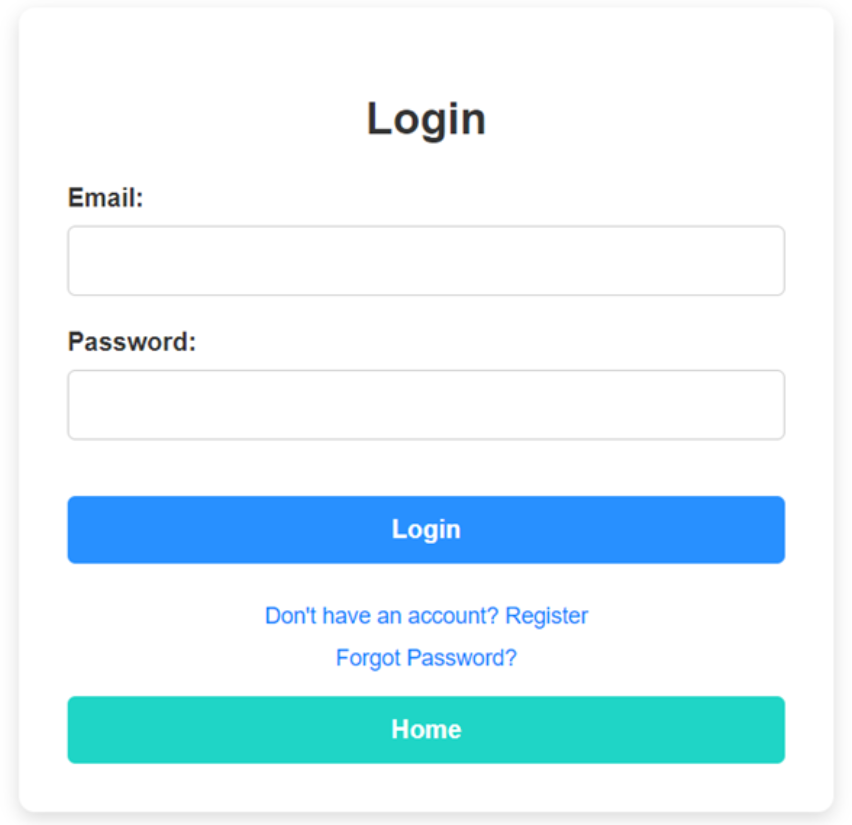
\includegraphics[width=0.4\textwidth]{assets/155}
	\caption*{\bfseries Рис. 5 - Форма авторизации}
\end{figure}


Переходя на страницу выбора определенного доктора, страница сведений о
враче предоставляет подробную информацию, включая его профиль и
назначения, отображен на Рисунке 6. При инициализации компонента данные
о враче извлекаются из параметров маршрута с использованием его
идентификатора. Метод системы получает информацию о профиле врача, такую
как имя, фамилия и адрес электронной почты. Если пользователь не
авторизован, он перенаправляется на страницу входа.

\begin{figure}[H]
	\centering
	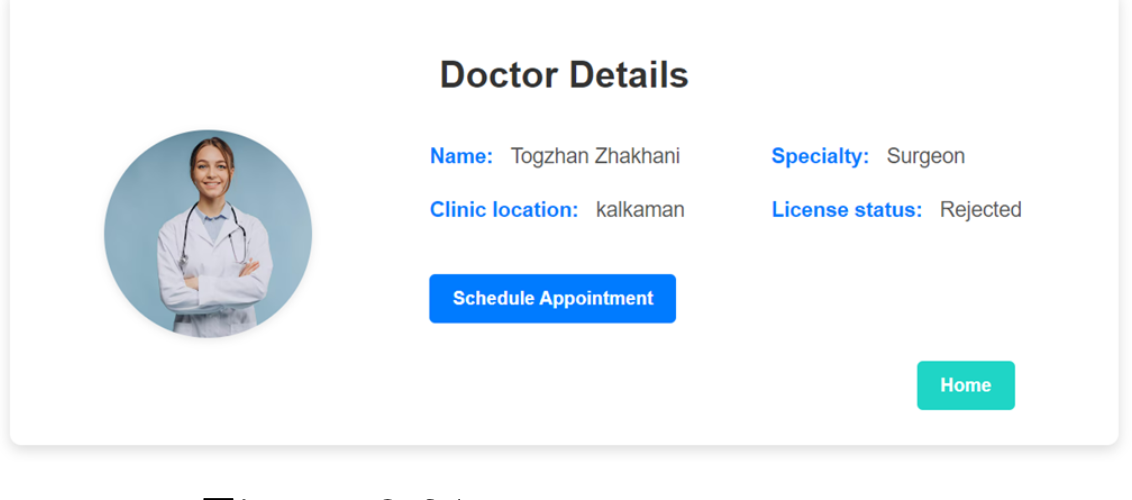
\includegraphics[width=0.8\textwidth]{assets/156}
	\caption*{\bfseries Рис. 6 - Профиль доктора}
\end{figure}


Управление встречами в системы Телемедицины является критическим
элементом, обеспечивающим плавное планирование, наблюдение и
регулирование встреч между врачами и пациентами. Система предоставляет
надежные функции, помогающие упростить все этапы взаимодействия, включая
создание, управление и интеграцию с внешними инструментами. Пользователи
имеют возможность выбирать доступные временные слоты из динамического
календаря, который отображает как свободные, так и зарезервированные
слоты, гарантируя прозрачность и легкость использования системы для
записи на консультацию на Рисунке 7.

\begin{figure}[H]
	\centering
	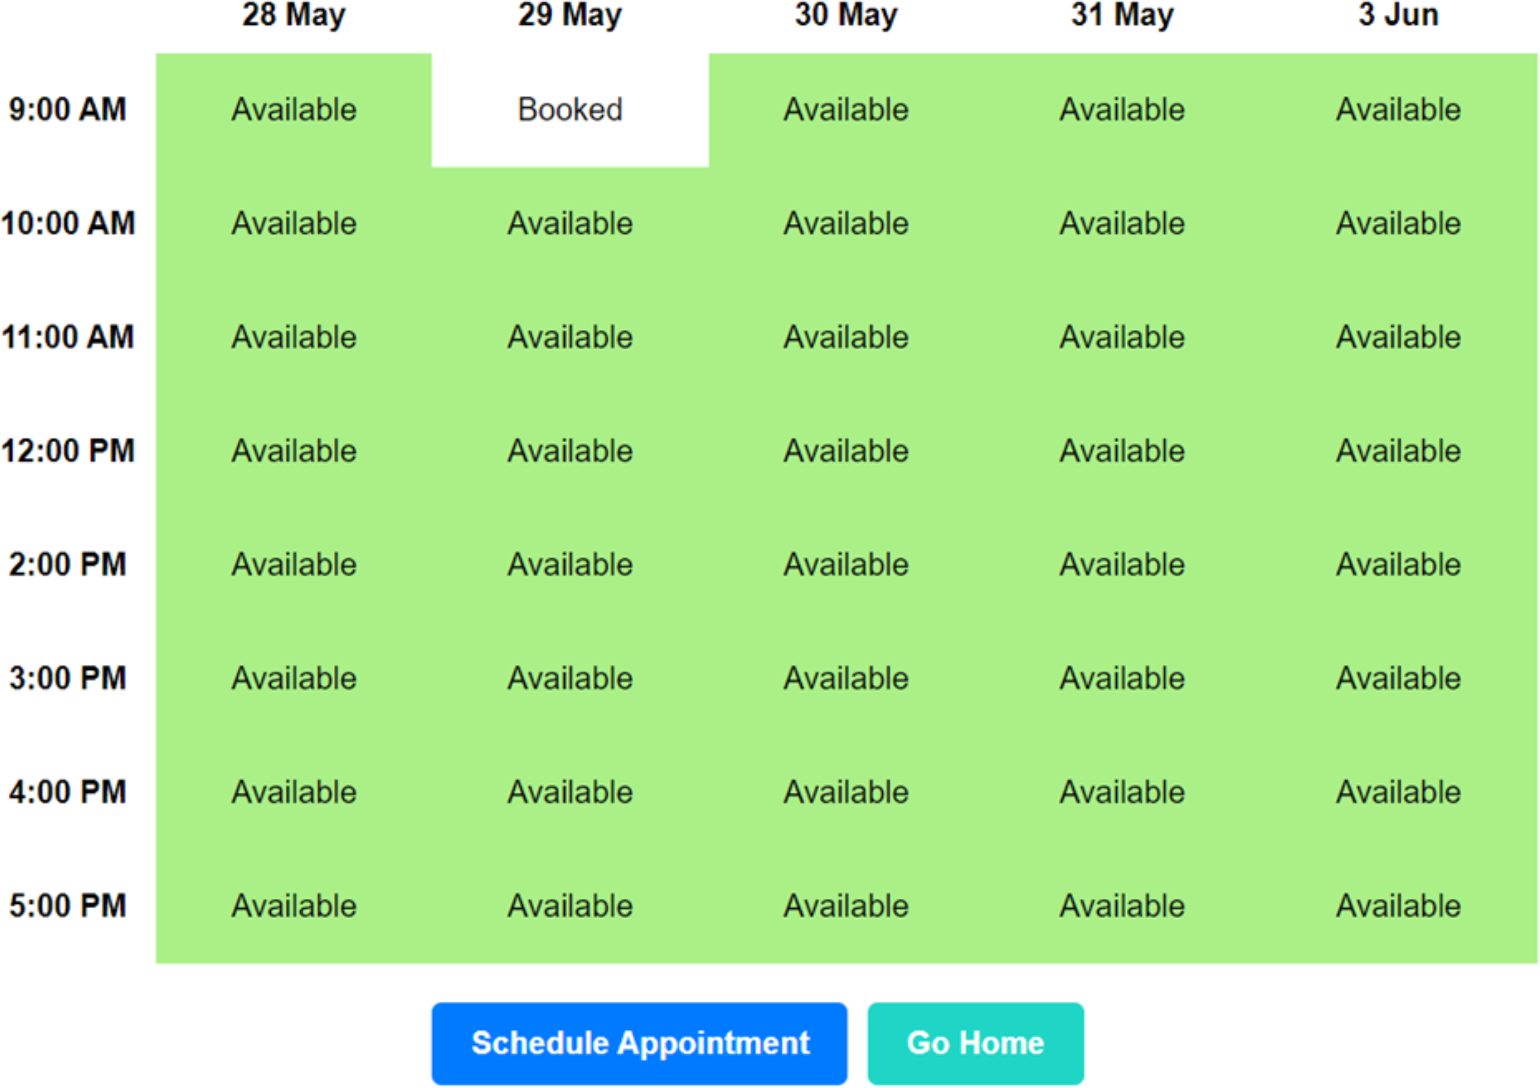
\includegraphics[width=0.8\textwidth]{assets/157}
	\caption*{\bfseries Рис. 7 - Страница планирования встреч}
\end{figure}


Функция планирования встреч в МИС проверяет выбранный интервал и
аутентификацию пользователя. Она извлекает идентификатор пациента и
формирует данные о встрече с использованием идентификатора врача. При
редактировании данные обновляются, при создании встречи они добавляются.
После успешного выполнения операции пользователь получает уведомление, а
при ошибке система предупреждает.

Разработка модели медицинской информационной системы для записи на прием
направлена на облегчение планирования встреч между медицинского
персонала и пациентов. Система обеспечивает удобный интерфейс для записи
на прием к врачу, управления расписанием и проведения медицинских
консультаций.

Для непрерывного улучшения системы существенно необходимо собирать
обратную связь от пользователей через опросы, фокус-группы или
индивидуальные интервью. Это позволит оценить их опыт, выявить узкие
места и определить приоритеты для будущих улучшений. Такой подход
приводит к повышению эффективности работы системы, улучшению качества
заботы о пациентах и обеспечивает бесперебойное функционирование.

{\bfseries Выводы.} В результате проведенного исследования была разработана
и предложена модель медицинской информационной системы (МИС) для
телемедицины, ориентированная на улучшение процесса записи пациентов к
медицинским специалистам. Основной целью данной работы было создание
решения, направленного на повышение качества медицинских услуг,
оптимизацию административных процессов и расширение доступа к
медицинским услугам для пациентов, особенно в удаленных регионах.

Для разработки системы использовались современные веб-технологии: Django
для серверной части, Angular для внешнего интерфейса и SQLite для
управления базами данных. Основные модули системы включают регистрацию и
аутентификацию пользователей, управление профилями пациентов и врачей, а
также планирование встреч.

Анализ производительности системы показал, что использование базы данных
SQLite позволяет эффективно обрабатывать записи пациентов и медицинских
специалистов. Однако SQLite ограничивает масштабируемость системы. Для
крупных медицинских учреждений с большим объемом данных и пользователей
необходимо перейти на более мощные системы управления базами данных.

Качественные показатели работы системы показывают, что улучшено
взаимодействие между пациентами и медицинским персоналом, а также
упрощен процесс записи. Однако текущая версия системы требует
дополнительных мер для усиления безопасности данных, что особенно важно
при работе с конфиденциальной медицинской информацией. Требуется
внедрение улучшенных механизмов аутентификации и верификации.

Система прошла апробацию медицинскими специалистами клиники «Aisera
Clinic» в городе Астана, где продемонстрировала свою эффективность и
надежность. Результаты апробации подтверждают, что внедрение МИС
способствует упрощению процессов записи и обработки информации о
пациентах, а также улучшению качества предоставляемых медицинских услуг.

В дальнейшем развитии системы планируется интеграция дополнительных
функций, усиление мер безопасности и улучшение пользовательского
интерфейса для более эффективного обслуживания пользователей и обработки
больших объемов данных. Также предусмотрено расширение системы для
крупных учреждений с применением более мощных баз данных и улучшенной
системы безопасности.

Таким образом, разработанная медицинская информационная система
представляет значительный прогресс в управлении медицинскими услугами,
предоставляя комплексное решение для записи на прием и
онлайн-консультаций. С постоянным развитием и адаптацией к изменяющимся
потребностям, МИС будет продолжать обеспечивать высокий уровень
эффективности и доступности медицинских услуг в условиях цифровой
трансформации здравоохранения.



\begin{center}
  {\bfseries Литература}
  \end{center}

\begin{noparindent}

\begin{enumerate}
\def\labelenumi{\arabic{enumi}.}
\item
  Giansanti D. Ten years of telehealth and digital healthcare: Where are
  we? //Healthcare. -- MDPI.- 2023. - Vol. 11. -- №. 6. DOI
  10.3390/healthcare11060875
\item
  Smith A. C., Thomas E., Snoswell C. L., Haydon H., Mehrotra A.,
  Clemensen J., and Caffery L.J. Telehealth for global emergencies:
  Implications for coronavirus disease 2019 (COVID-19) //Journal of
  telemedicine and telecare.- -2020.-Vol.26(5).- P. 309-313. DOI 10.1177/1357633X20916567
\end{enumerate}


\begin{enumerate}
\def\labelenumi{\arabic{enumi}.}
\setcounter{enumi}{2}
\item
  Betancourt J. A., Rosenberg M. A., Zevallos A., Brown J. R., and
  Mileski M. The impact of COVID-19 on telemedicine utilization across
  multiple service lines in the United States //Healthcare. -- MDPI.-
  2020. -Vol. 8(4). \\DOI 10.3390/healthcare8040380
\item
  Alotaibi Y. K., Federico F. The impact of health information
  technology on patient safety //Saudi medical journal. - 2017. -Vol.
  38(12). - P. 1173-1180. DOI 10.15537/smj.2017.12.20631
\item
  Phuong J., Ordóñez P., Cao J., Moukheiber M., Moukheiber L., Caspi A.,
  and Mankoff J. Telehealth and digital health innovations: A mixed
  landscape of access //PLOS Digital Health. -- 2023. - Vol. 2(12). DOI
  10.1371/journal.pdig.0000401
\item
  Ma Y., Zhao C., Zhao Y., Lu J., Jiang H., Cao Y., and Xu Y.
  Telemedicine application in patients with chronic disease: a
  systematic review and meta-analysis //BMC medical informatics and
  decision making. - 2022. -Vol. 22(1). DOI 10.1186/s12911-022-01845-2.
\item
  Seitenov A., Zhukabayeva T., Sansyzbay K., Kalpakov E. Design
  development of medicine information system for telemedicine field
  //The Bulletin of KazATC.- 2023. -Vol. 127(4).- P. 241-251. DOI
  10.52167/1609-1817-2023-127-4-241-251
\end{enumerate}

Akhtar M. N., Haleem A., Javaid M. Scope of health care system in rural
areas under Medical 4.0 environment //Intelligent Pharmacy.- 2023. -Vol.
1(4). - P. 217-223. DOI 10.1016/j.ipha.2023.07.003

\begin{enumerate}
\def\labelenumi{\arabic{enumi}.}
\setcounter{enumi}{7}
\item
  Kim Y.S. Telemedicine in the USA with focus on clinical applications
  and issues //Yonsei medical journal. -2004.- Vol. 45(5).- P. 761-775.
  DOI 10.3349/ymj.2004.45.5.761
\item
  Shen Y.T., Che L., Yue W.W., and Xu H.X. Digital technology-based
  telemedicine for the COVID-19 pandemic //Frontiers in medicine. -
  2021.-Vol. 8. DOI 10.3389/fmed.2021.646506
\item
  Epizitone A., Moyane S.P., Agbehadji I.E. A systematic literature
  review of health information systems for healthcare //Healthcare.-
  MDPI.-2023.-Vol. 11(7). DOI 10.3390/healthcare11070959
\end{enumerate}


\begin{enumerate}
\def\labelenumi{\arabic{enumi}.}
\setcounter{enumi}{10}
\item
  Palozzi G., Schettini I., Chirico A. Enhancing the sustainable goal of
  access to healthcare: findings from a literature review on
  telemedicine employment in rural areas //Sustainability. -- 2020. -
  Vol. 12(8). DOI 10.3390/su12083318
\item
  Combi C., Pozzani G., Pozzi G. Telemedicine for developing countries.
  A Survey and Some Design Issues //Applied Clinical Informatics.-2016.
  -Vol. 7(4). - P. 1025-1050. DOI 10.4338/ACI-2016-06-R-0089
\end{enumerate}



\begin{enumerate}
\def\labelenumi{\arabic{enumi}.}
\setcounter{enumi}{12}
\item
  Shigekawa E., Fix M., Corbett G., Roby D. H., and Coffman, J. The
  current state of telehealth evidence: a rapid review //Health
  Affairs.-2018. --Vol. 37(12) -P. 1975-1982.
\end{enumerate}

DOI 10.1377/hlthaff.2018.05132

\begin{enumerate}
\def\labelenumi{\arabic{enumi}.}
\setcounter{enumi}{13}
\item
  Dullet N.W. Geraghty E.M., Kaufman T., Kissee J.L., King J., Dharmar
  M., and Marcin J.P. Impact of a university-based outpatient
  telemedicine program on time savings, travel costs, and environmental
  pollutants //Value in Health. -- 2017. -- Vol. 20(4). -- P. 542-546.
  DOI 10.1016/j.jval.2017.01.014
\item
  De La Torre-Díez I. López-Coronado M., Vaca C., Aguado J. S., and de
  la Torre B. Cost-utility and cost-effectiveness studies of
  telemedicine, electronic, and mobile health systems in the literature:
  a systematic review //Telemedicine and e-Health. -2015.-Vol. 21(2).
  -P. 81-85. DOI 10.1089/tmj.2014.0053
\end{enumerate}



\begin{enumerate}
\def\labelenumi{\arabic{enumi}.}
\setcounter{enumi}{15}
\item
  Agarwal S., LeFevre A. E., Lee J., L'engle K., Mehl G., Sinha C., \&
  Labrique, A. Guidelines for reporting of health interventions using
  mobile phones: mobile health (mHealth) evidence reporting and
  assessment (mERA) checklist. //bmj. - 2016. -Vol. 352. DOI
  10.1136/bmj.i1174
\item
  Garg, A. What is Angular?: Syntax, Features, Architecture, \& More:
  Internshala Trainings Blog. \\DOI 10.1089/tmj.2014.0053- URL:  https://trainings.internshala.com/blog/what-is-angular/
\item
  Priy S. Introduction to SQLite. // GeeksforGeeks.
  URL: https://www.geeksforgeeks.org/introduction-to-sqlite/
\end{enumerate}

\end{noparindent}

\emph{{\bfseries Сведения об авторах}}
\begin{noparindent}

Сейтенов А.С. - докторант, Евразийский национальный университет им. Л.
Н. Гумилева, Астана, Казахстан, e-mail: altynbekss@gmail.com;

Жукабаева Т.К. - PhD, профессор Евразийский национальный университет им.
Л. Н. Гумилева, Астана, Казахстан,e-mail: tamara.kokenovna@gmail.com;

Al-Majeed S. - PhD, профессор, Al Akhawayn University, Ифран, Марокко,
e-mail: salah.almajeed@gmail.com;

Wolff C. - PhD, профессор, Fachhochschule Dortmund, Дортмунд,
Германия,,e-mail: carsten.wolff@fh-dortmund.de
\end{noparindent}

\emph{{\bfseries Information about the authors}}
\begin{noparindent}

Seitenov A.S. - PhD student, L.N.Gumilyov Eurasian National University,
Astana, Kazakhstan, e-mail: altynbekss@gmail.com;

Zhukabayeva T.K. - PhD, professor, L.N.Gumilyov Eurasian National
University, Astana, Kazakhstan, \\e-mail: tamara.kokenovna@gmail.com;

Al-Majeed S. - PhD, professor, Al Akhawayn University, Ifrane, Morocco,
e-mail: salah.almajeed@gmail.com;

Wolff C. - PhD, professor, Fachhochschule Dortmund, Dortmund, Germany,
e-mail: carsten.wolff@fh-dortmund.de
\end{noparindent}
